%%% Research Diary - Entry
%%% Template by Mikhail Klassen, April 2013

\documentclass[11pt,letterpaper]{article}
\usepackage{float}
\usepackage{researchdiary_png}
\newcommand{\workingDate}{\textsc{2025 $|$ April }}
\newcommand{\userName}{Charalampos Papadopoulos}
\newcommand{\institution}{National Technical University of Athens}

\begin{document}
\univlogo

\title{PLL Simulations Logbook}
\vspace{0.5cm}
{\Huge Προσομοιώσεις PLL με ιδανικά στοιχεία}\\[5mm]

Στην παρούσα αναφορά θα προσομοιώσουμε το PLL στο LTSpice και θα ελέγξουμε τις δυνατότητες της σχεδίασης μας.\\[2mm]

\section*{1. Αρχικό Κύκλωμα}
Το schematic του PLL φαίνεται στο Σχήμα~\ref{fig:pll_schematic}.

\begin{figure}[H]
    \centering
    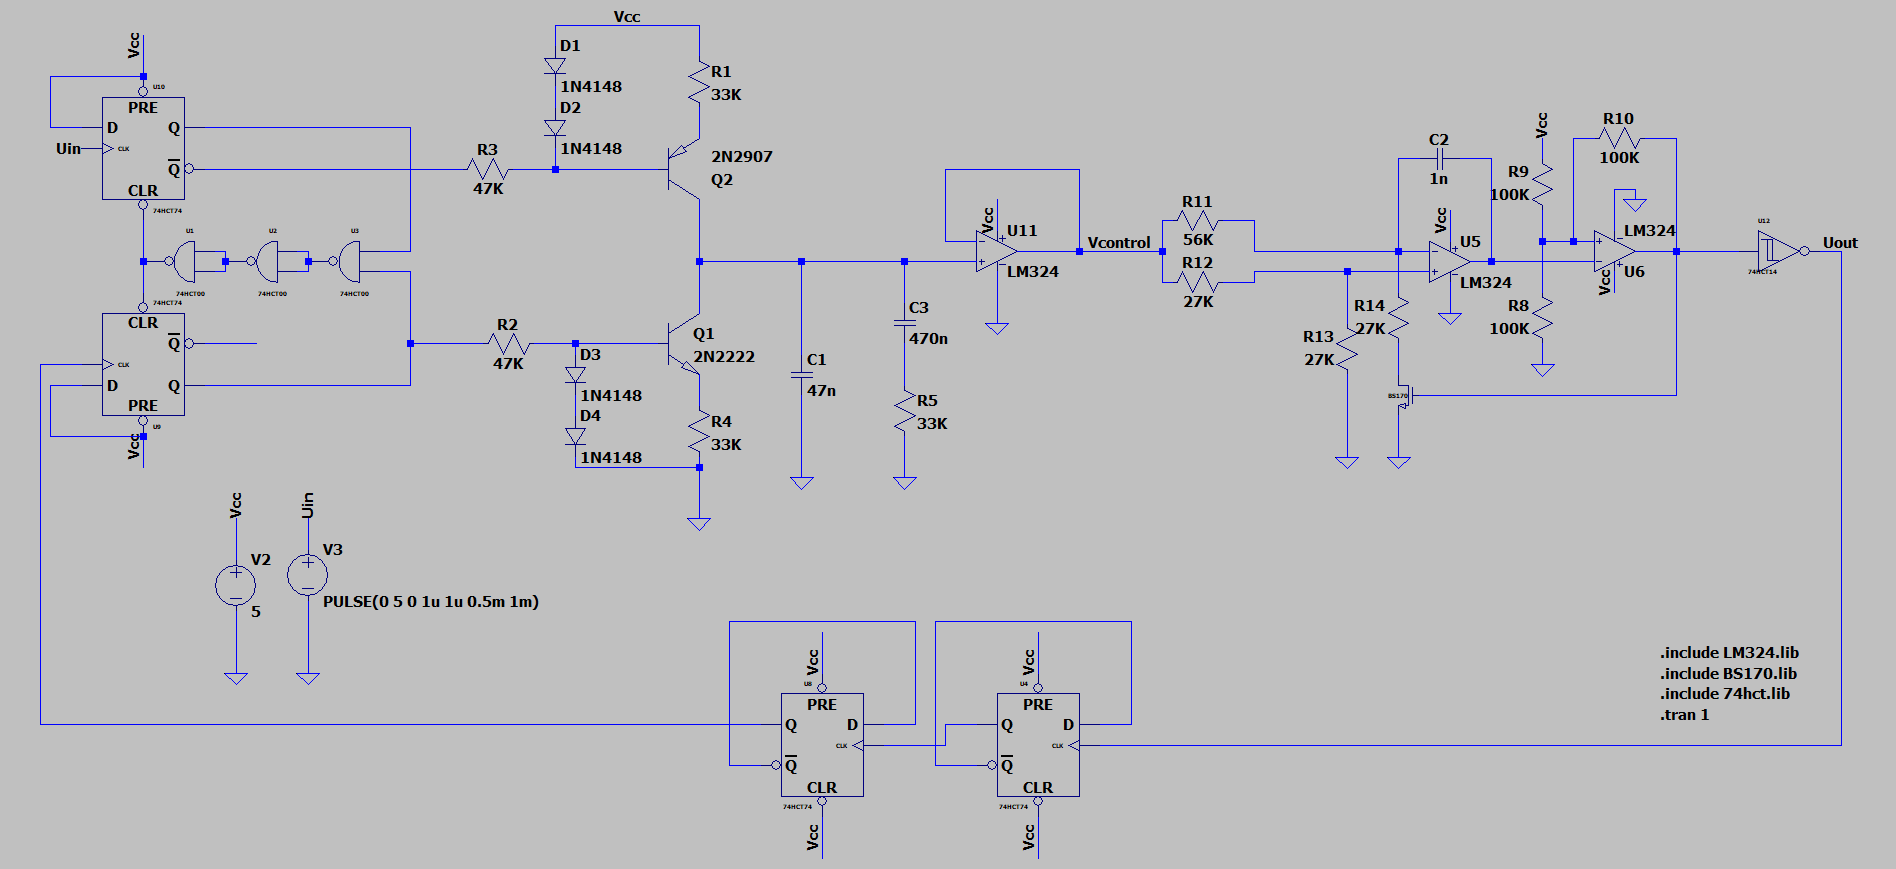
\includegraphics[width=\textwidth]{figures/pll.png}
    \caption{PLL Schematic}
    \label{fig:pll_schematic}
\end{figure}

\section*{2. Προσομοίωση για U\textsubscript{in} = 1 kHz}
Κατά την αρχική προσομοίωση (Σχήμα~\ref{fig:pll_simulation_1khz}), για \( U_{in} = 1\,\text{kHz} \), παρατηρείται πολύ καλό κλείδωμα στα 100 ms, με \( V_{control} = 1.4\,\text{V} \) και τετραπλασιασμό της συχνότητας στην έξοδο.

\begin{figure}[H]
    \centering
    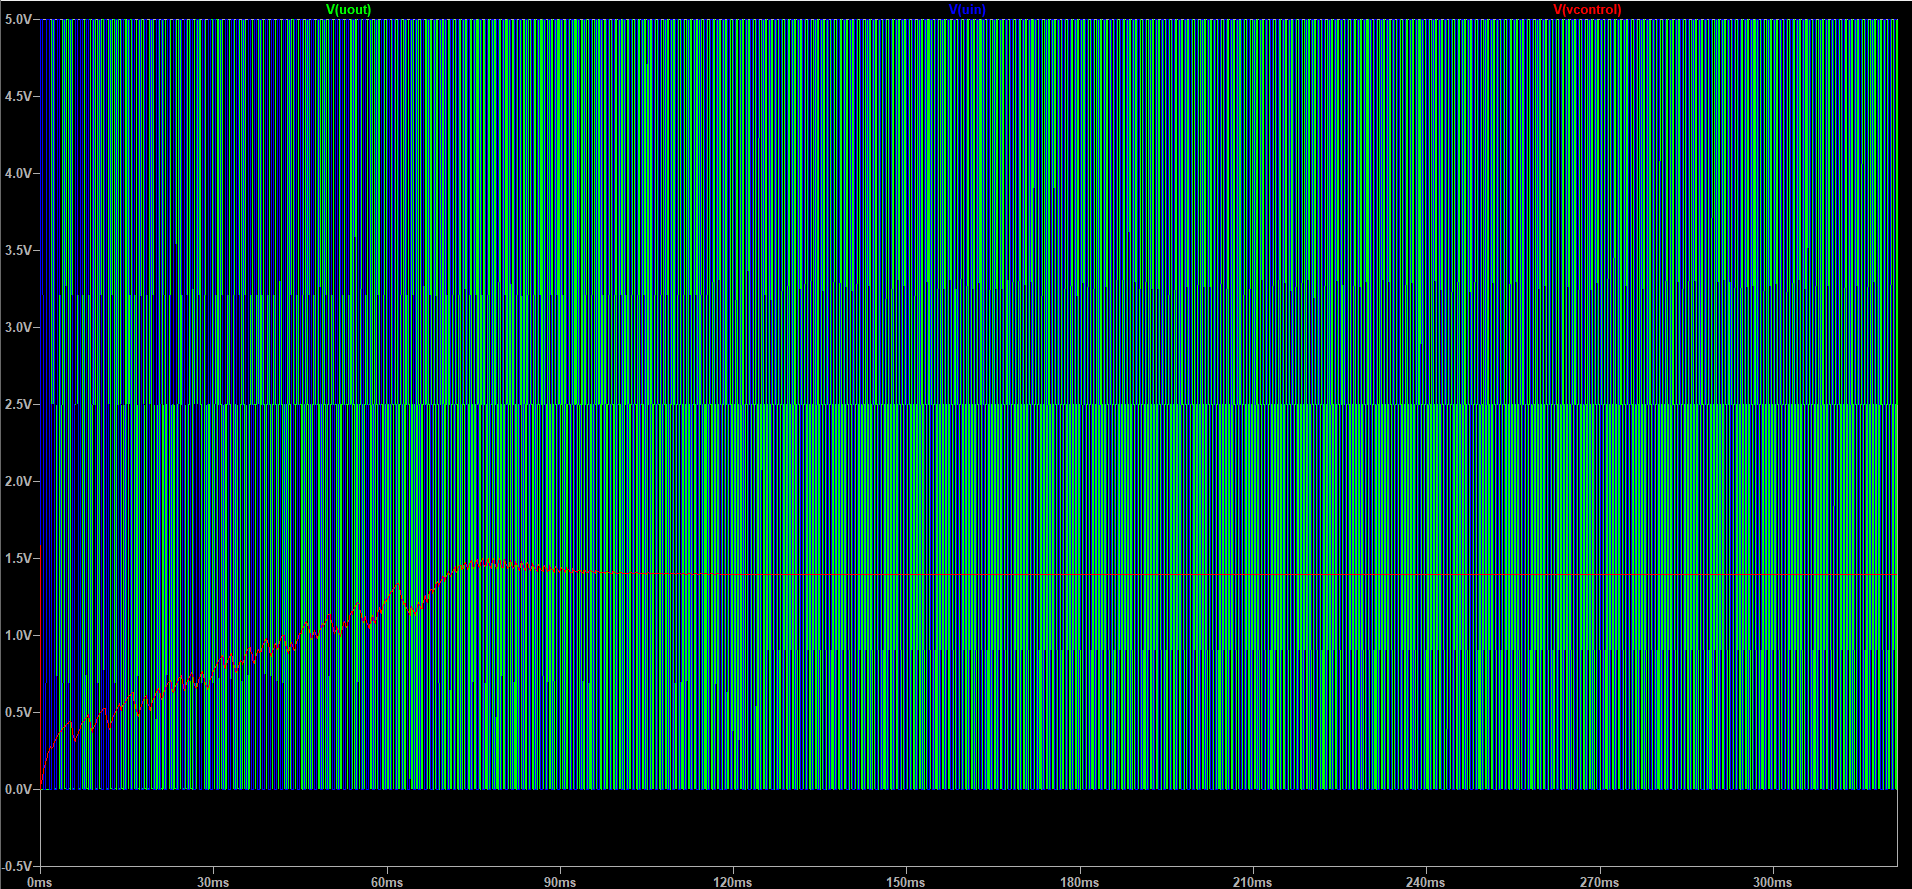
\includegraphics[width=\textwidth]{figures/sim1.png}
    \caption{PLL Simulation for \( U_{in} = 1\,\text{kHz} \)}
    \label{fig:pll_simulation_1khz}
\end{figure}

\section*{3. Προσομοίωση για U\textsubscript{in} = 1.2 kHz}
Αυξάνοντας τη συχνότητα εισόδου στα 1.2 kHz — όριο κλειδώματος του PLL στο εργαστήριο — το κύκλωμα συνεχίζει να κλειδώνει, με \( V_{control} = 2\,\text{V} \) (Σχήμα~\ref{fig:pll_simulation_1.2khz}).

\begin{figure}[H]
    \centering
    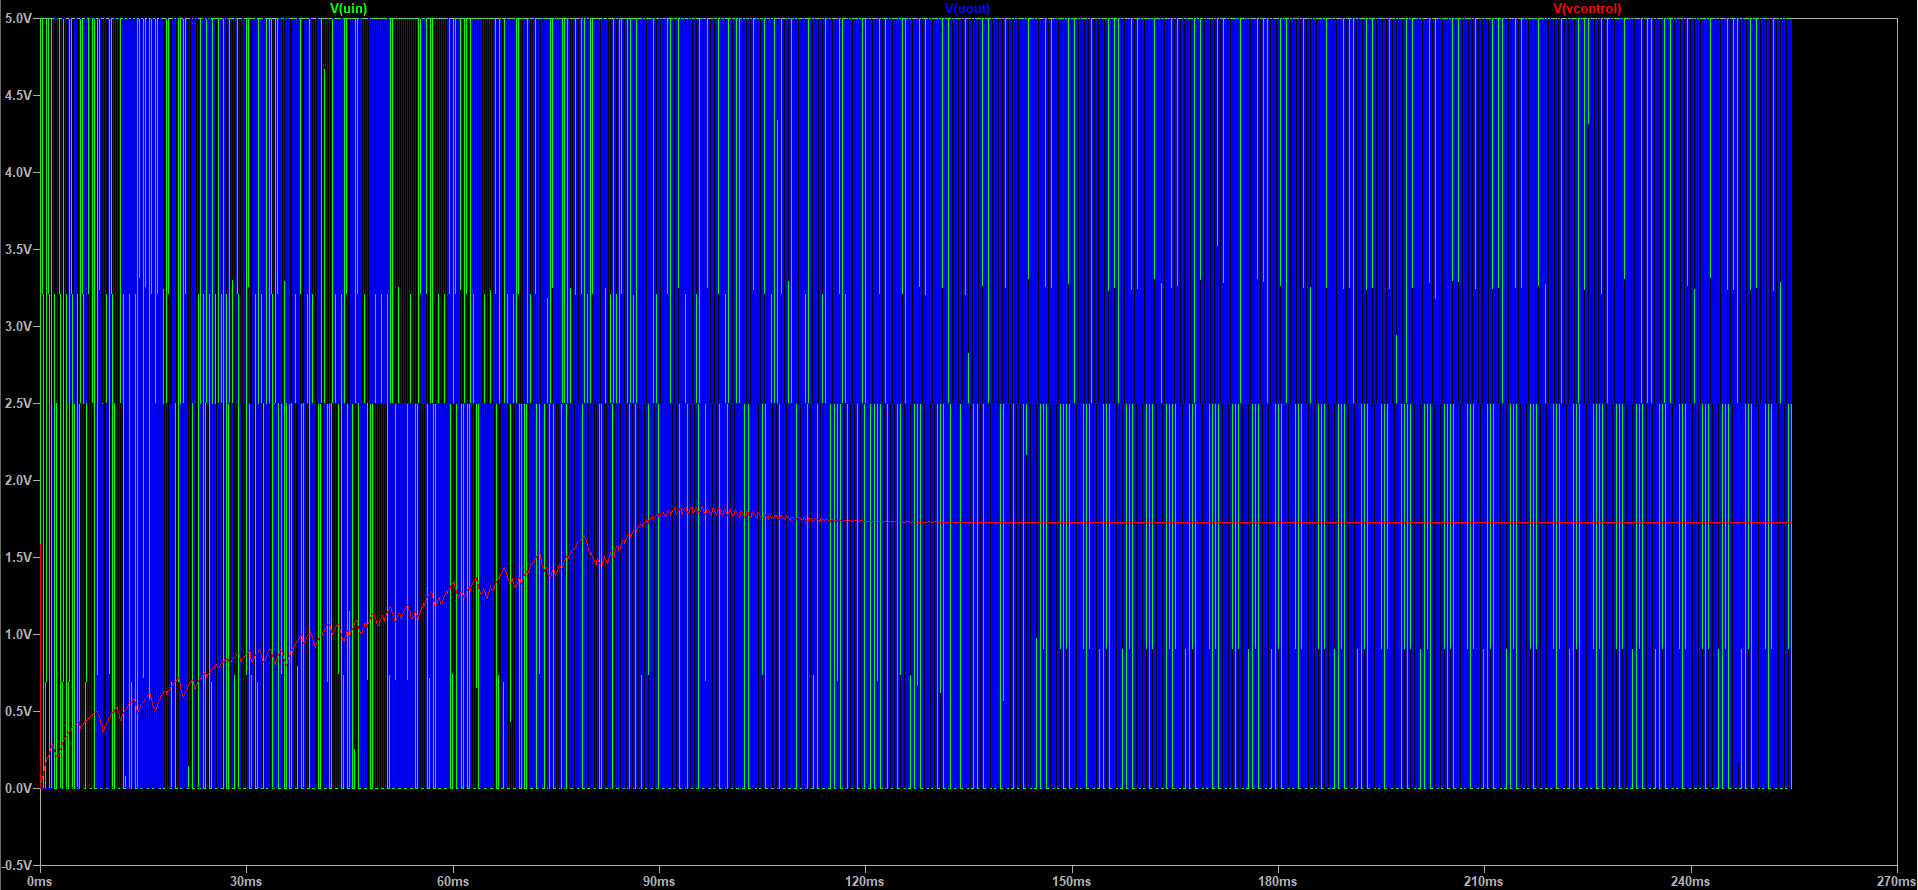
\includegraphics[width=\textwidth]{figures/sim2.png}
    \caption{PLL Simulation for \( U_{in} = 1.2\,\text{kHz} \)}
    \label{fig:pll_simulation_1.2khz}
\end{figure}

\section*{4. Προσομοίωση για U\textsubscript{in} = 1.5 kHz}
Για \( U_{in} = 1.5\,\text{kHz} \), το PLL εξακολουθεί να κλειδώνει, με \( V_{control} = 3\,\text{V} \). Εδώ αρχίζει να φαίνεται η διαφορά μεταξύ προσομοίωσης και πραγματικού κυκλώματος.

\begin{figure}[H]
    \centering
    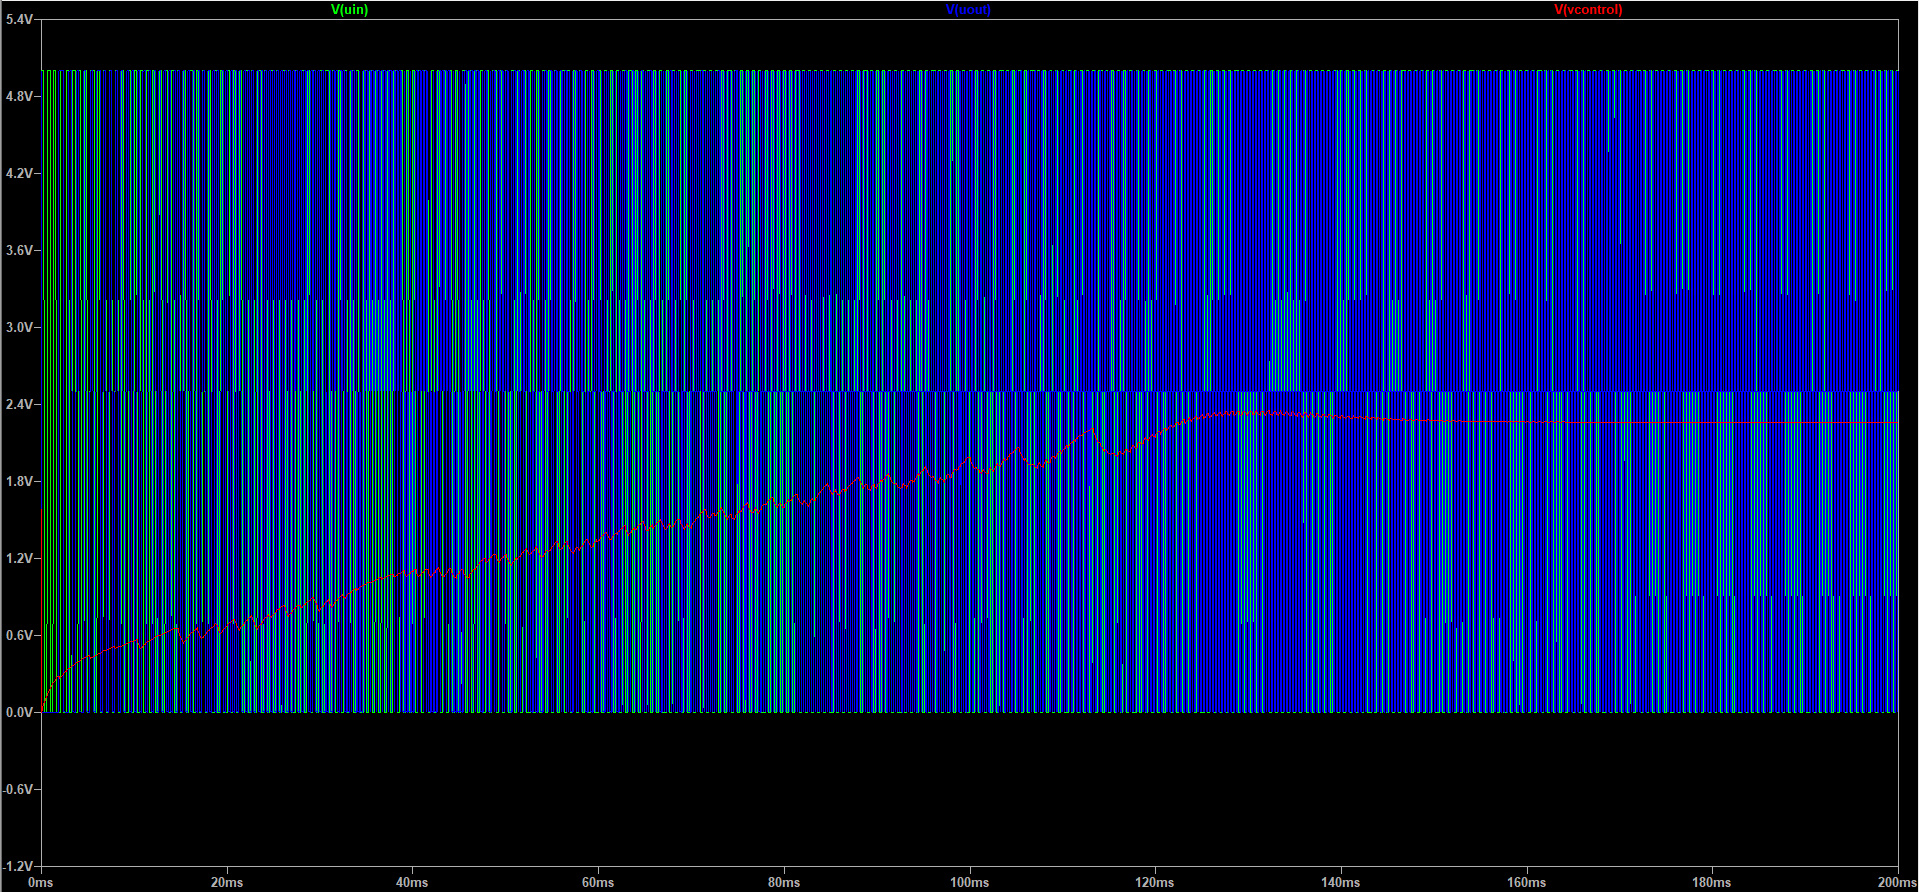
\includegraphics[width=\textwidth]{figures/sim3.png}
    \caption{PLL Simulation for \( U_{in} = 1.5\,\text{kHz} \)}
    \label{fig:pll_simulation_1.5khz}
\end{figure}

\section*{5. Προσομοίωση για U\textsubscript{in} = 2.5 kHz}
Αυξάνοντας τη συχνότητα εισόδου στα 2.5 kHz, παρατηρούμε ότι το PLL \textbf{δεν} κλειδώνει πλέον. Το \( V_{control} \) φτάνει στα 3.5 V και σταθεροποιείται (Σχήμα~\ref{fig:pll_simulation_2.5khz}), κάτι που μοιάζει με κλείδωμα αλλά είναι παραπλανητικό.
Στην πραγματικότητα, ο ενισχυτής φτάνει την τάση κορεσμού, η οποία είναι περίπου 1.4–1.6 V χαμηλότερη από την τάση τροφοδοσίας.

\begin{figure}[H]
    \centering
    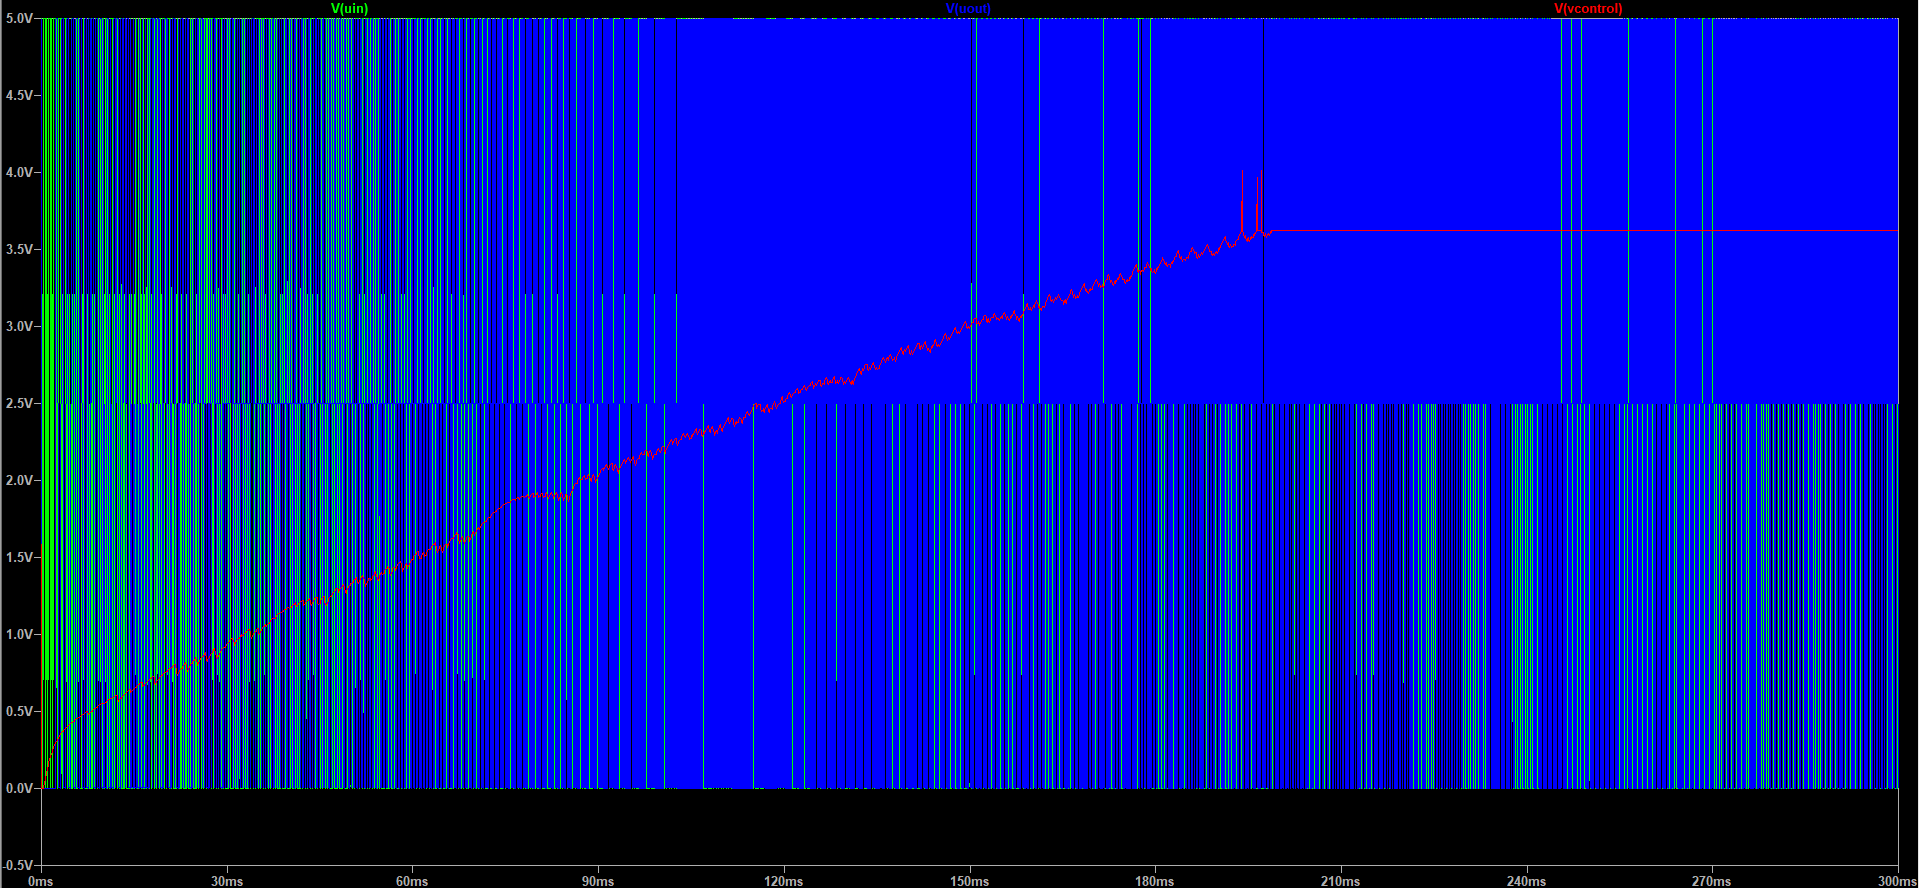
\includegraphics[width=\textwidth]{figures/sim4.png}
    \caption{PLL Simulation for \( U_{in} = 2.5\,\text{kHz} \)}
    \label{fig:pll_simulation_2.5khz}
\end{figure}


\section*{6. Αύξηση Τάσης Τροφοδοσίας στα 6V}
Δοκιμάζουμε να αυξήσουμε την τάση τροφοδοσίας στα 6 V. 
    Το \( V_{control} \) φτάνει στα 4.5 V αλλά το PLL \textbf{εξακολουθεί να μην κλειδώνει} (Σχήμα~\ref{fig:pll_simulation_2.5khz_6v}). Δεν παρατηρείται διαφορά ούτε με αποσύνδεση του ST και του διαιρέτη.

\begin{figure}[H]
    \centering
    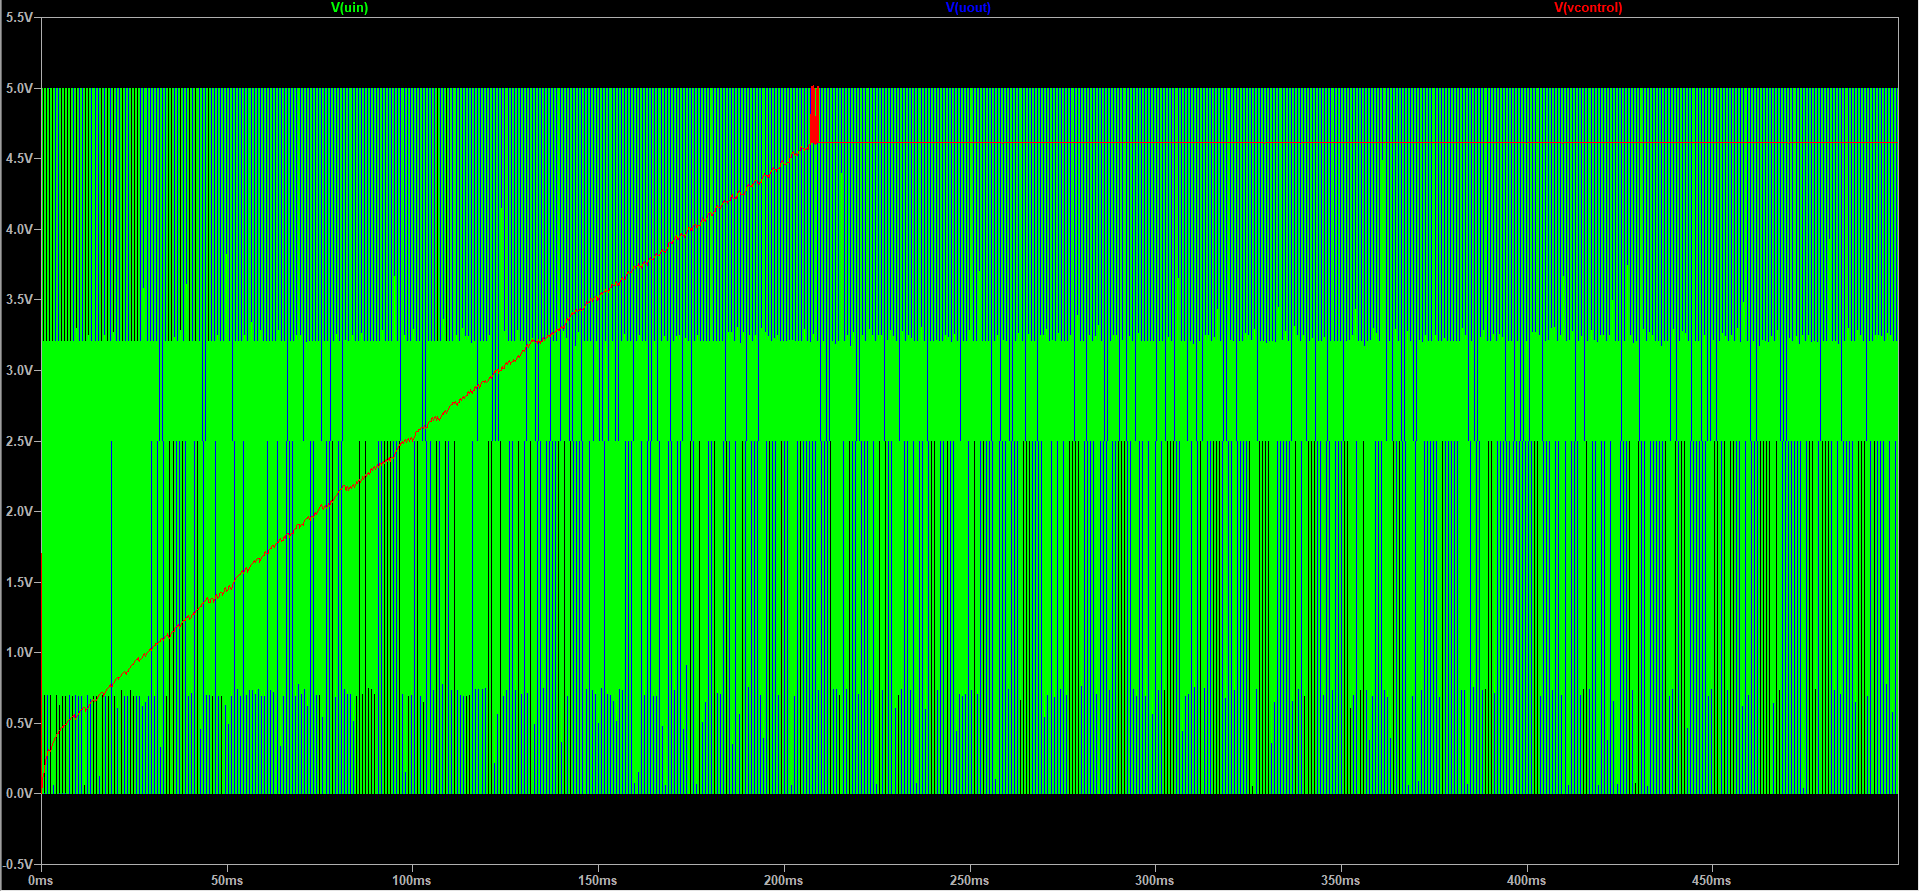
\includegraphics[width=\textwidth]{figures/sim5.png}
    \caption{PLL Simulation for \( U_{in} = 2.5\,\text{kHz} \), \( V_{cc} = 6\,\text{V} \)}
    \label{fig:pll_simulation_2.5khz_6v}
\end{figure}

\section*{7. Χρήση Ιδανικού OpAmp}
Αντικαθιστούμε τον OPAMP U11 (buffer) με τον ιδανικό `universalOpAmp`. Το κύκλωμα κλειδώνει, με \( V_{control} = 4.5\,\text{V} \) (Σχήμα~\ref{fig:pll_simulation_2.5khz_ideal_opamp}). Όμως, πλέον βρισκόμαστε πολύ κοντά στην τάση τροφοδοσίας, περιορίζοντας τη δυνατότητα περαιτέρω αύξησης συχνότητας.

\begin{figure}[H]
    \centering
    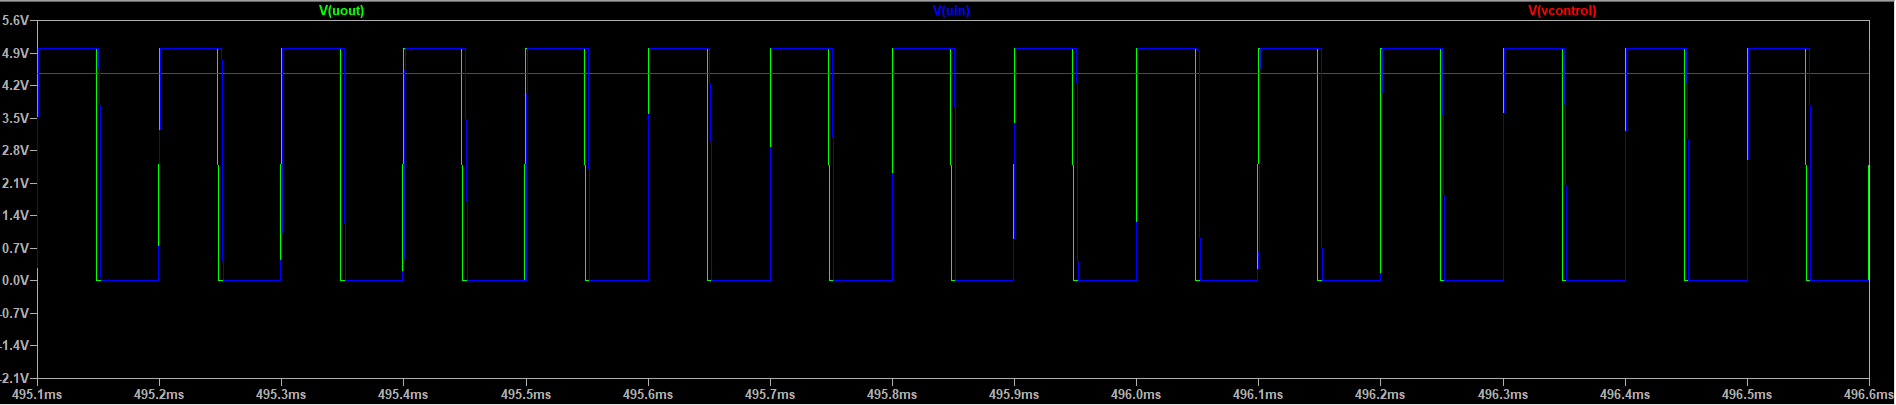
\includegraphics[width=\textwidth]{figures/sim6.png}
    \caption{PLL Simulation for \( U_{in} = 2.5\,\text{kHz} \) with Ideal OpAmp}
    \label{fig:pll_simulation_2.5khz_ideal_opamp}
\end{figure}

\section*{8. Αντικατάσταση Όλων με Ιδανικά Στοιχεία}
Αντικαθιστούμε όλους τους ενισχυτές με `universalOpAmp2` και τα τρανζίστορ με ιδανικά. Δεν παρατηρείται βελτίωση — αντίθετα, \textbf{το κύκλωμα δεν κλειδώνει ούτε στα 10 kHz}.

Το συμπέρασμα είναι πως η τοπολογία του VCO είναι ο περιοριστικός παράγοντας. Απαιτεί υψηλές τάσεις για να παραγάγει παλμούς (σχετικά) χαμηλής συχνότητας.

\end{document}
